%\documentclass[10pt,a4paper]{article}
\documentclass[12pt,a4paper]{article}
\usepackage{graphicx,amsmath}
%\usepackage{subfigure}
\usepackage{float}
\usepackage[german]{babel}
\usepackage[utf8]{inputenc}
\setcounter{secnumdepth}{4}
\usepackage[top=2cm, bottom=2.5cm, left=3cm, right=3cm]{geometry}
\usepackage{subcaption}
\begin{document}


%\title{Bachelorarbeit}
%\author{Richard Kullmann}
%\date{02.06.2017}

\thispagestyle{empty}
%\setcounter{page}{2}
\newpage
\tableofcontents
\thispagestyle{empty}
\newpage
\pagenumbering{arabic}
\section{Burstende Neuronen}
\begin{figure}[H]
	\centering
	\begin{subfigure}{.45\textwidth}
		\centering
		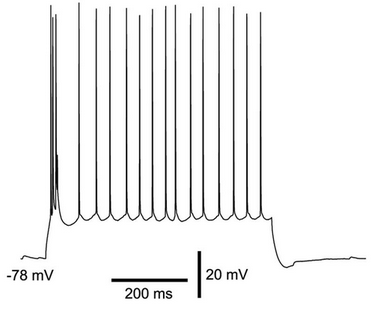
\includegraphics[scale=0.4]{25.png}
		\caption*{Spike Train eines intrinsisch burstenden Neurons $^1$}
		\label{fig25}
	\end{subfigure}\hspace{5mm}%
	\begin{subfigure}{.45\textwidth}
		\centering
		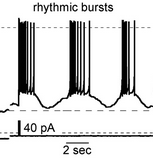
\includegraphics[scale=0.8]{26.png}
		\caption*{Periodisches Bursten in Nervenzellen aus dem Subthalamus $^2$}
		\label{fig26}
	\end{subfigure}
\end{figure}
\begin{figure}[H]
	\centering
	\begin{subfigure}{.45\textwidth}
		\centering
		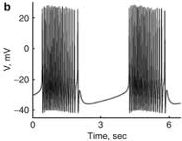
\includegraphics[scale=0.8]{27.png}
		\caption*{
			Parabolisches Bursten im Morris-Lecar-Modell, wobei die langsame Oszilation durch einen zus"atzlichen langsamen Ca-Strom entsteht $^3$}
		\label{fig27}
	\end{subfigure}\hspace{5mm}%
	\begin{subfigure}{.45\textwidth}
		\centering
		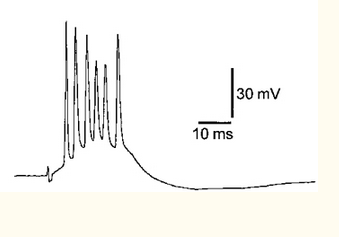
\includegraphics[scale=0.48]{42.png}
		\caption*{
			In-vitro Aufnahme von Lamina V Pyramidenzellen von Ratten $^4$}
		\label{fig42}
	\end{subfigure}
\end{figure}
\begin{figure}[H]
	\centering
	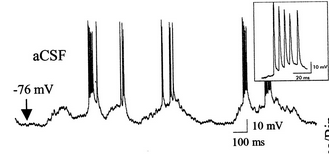
\includegraphics[scale=.8]{28.png}
	\caption*{In-vivo Messung des Spike Trains einer Nervenzelle im Gehirn $^5$}
	\label{fig28}
\end{figure}
\footnotetext[1]{Zhong-Wei Zhang, "Maturation of Layer V Pyramidal Neurons in the Rat Prefrontal Cortex: Intrinsic
	Properties and Synaptic Function,"\textit{J Neurophysiol. 91}, 2004.}
\footnotetext[2]{Jason I. Kass and Isabelle M. Mintz, "Silent plateau potentials, rhythmic bursts, and pacemaker firing: Three patterns of activity that coexist in quadristable subthalamic 		neurons,"\textit{PNAS Vol. 103}, 2006.}
\footnotetext[3]{David Fox et al.,"Bursting in Neurons and Small Networks,"\textit{Encyclopedia of Computational Neuroscience}, 2014.}
\footnotetext[4]{Stephen R. Williams and Greg J. Stuart,"Mechanisms and consequences of action potential burst firing in rat neocortical pyramidal neurons,"\textit{J Physiol 521}, 1999.}
\footnotetext[5]{A. R. West et al.,"Direct Examination of Local Regulation of Membrane Activity in Striatal and Prefrontal Cortical Neurons in Vivo Using Simultaneous 		Intracellular Recording and Microdialysis,"\textit{J Pharmacol Exp Ther. 301}, 2002.}
\newpage
Bursten beschreibt ein Ph"anomen in den Spike Trains von Nervenzellen, bei dem sich Perioden mit hochfrequentem Feuern und Ruhephasen abwechseln. Die schnellsten neuralen Oszillationen im menschlichen Gehirn sind die sogenannten Gamma-Wellen mit Frequenzen zwischen 25 und 100 Hz. "Ahnliche Frequenzen sind auch in anderen Papern "uber burstende Neuronen zu finden \footnote[6]{K. Nakajima et al.,"Dynamic characteristics of a simplebursting neuron model,"\textit{NOLTA Vol. 3}, 2012.}\footnote[7]{
X. Zhao et al.,"Low dimensional model of bursting neurons,"\textit{J Comput Neurosci}, 2014. }. Daher wurden die Parameter des hier betrachteten Modells so gew"ahlt, dass die Neuronen im burstenden Zustand mit einer Frequenz von 70 Hz feuern.

\section{Absch"atzung des Spektrums}
Wie in $Theory\: of\: Stochastic\: Resonance$ beschrieben, erf"ahrt ein bistabiles System, welches einer periodischen Modulation unterliegt, auch eine Modulation in den "Ubergangsraten zwischen seinen beiden Zust"anden:
\begin{equation}
r_\pm(t)=f(\mu\pm\eta_0\cos(\omega_s t))
\end{equation}
$\mu$ ist hierbei das Verh"altnis $\Delta U/Q$ aus der Potentialbarriere zwischen den Zust"anden und der Rauschintensit"at. Der Parameter $\eta_0$ ist ein Ma"s f"ur die St"arke der Modulation. Mit dieser Annahme kann man das Spektrum mit folgender N"aherung beschreiben:
\begin{eqnarray}
S(\Omega)=\left(1-\frac{\alpha_1^2\eta_0^2}{2(\alpha_0^2+\omega_s^2)}\right)\left(\frac{4c^2\alpha_0}{\alpha_0^2+\Omega^2}\right)+\frac{\pi c^2\alpha_1^2\eta_0^2}{\alpha_0^2+\omega_s^2}\delta(\Omega-\omega_s)
\end{eqnarray}
Dabei ist $c^2$ die Varianz des ungest"orten, als symmetrisch angenommenen Zwei-Zustands-Systems und die Funktion $f$ wurde unter Annahme einer kleinen St"orung durch die ersten beiden Terme seiner Reihendarstellung angen"ahert, wobei:
\begin{align*}
\frac{1}{2}\alpha_0&=f(\mu)\\
\frac{1}{2}\alpha_1&=-\frac{d}{d\mu}f(\mu)
\end{align*} 
Das hier betrachtete bistabile System mit St"orung ist das $I_{Na,p}+I_K$-Modell:
	\begin{align*}
	C\dot{V} &= I - g_L(V-E_L) - g_{Na}m_{\infty}(V)(V-E_{Na}) - g_Kn(V-E_K)+\sqrt{2D}\xi(t)+\epsilon\cos(\omega_s t+\phi_i)\\
	\dot{n} &= (n_{\infty}(V)-n)/\tau(V)
	\end{align*}
Die Phase $\phi_i$ wird zuf"allig erzeugt und die Simulationen werden "uber mehrere verschiedene Phasen gemittelt.\\ Die Steady-State-Aktivierungsfunktion ist:
	\begin{align*}
	f_{\infty}(V) = \frac{1}{1+\exp\{(V_{1/2}-V)/k\}}
	\end{align*}
Die "Ubergangsraten wurden f"ur dieses System bisher mit Arrhenius-Gleichungen angen"ahert:
\begin{eqnarray}
r_{\pm}=r_{0,\pm}\text{e}^{-\frac{\Delta U_{\pm}}{Q}}
\end{eqnarray}
Um die oben beschriebene Formel anwenden zu k"onnen, m"ussen die beiden Raten im ungest"orten System identisch sein, also
\begin{eqnarray}
r_{\pm}=r_0\text{e}^{-\frac{\Delta U}{Q}}=r_0\text{e}^{-\mu}
\end{eqnarray}
Die Potentialbarrieren m"ussen durch zwei Geraden mit betraglich gleichem Anstieg beschrieben werden:
\begin{equation}
	\Delta U_\pm=\pm a\cdot I +b_\pm
\end{equation}
Die Potentialbarriere f"ur den "Ubergang vom burstenden zum ruhenden Zustand nimmt also mit $I$ zu, w"ahrend die Barriere f"ur den gegens"atzlichen "Ubergang abnimmt.\\
Aus dieser Darstellung folgt nun f"ur die Amplitude $\eta_0$:
\begin{eqnarray}
\eta_0=\frac{a\epsilon}{Q}
\end{eqnarray} 
Des weiteren erh"alt man f"ur die ersten beiden Vorfaktoren der Taylor-Reihe:
\begin{align*}
\alpha_0=\alpha_1=2r_0\text{e}^{-\frac{\Delta U}{Q}}
\end{align*}
Die Varianz der Feuerrate wird zun"achst nur numerisch aus dem Verlauf der Membranspannung bestimmt. Dann erh"alt man folgendes Spektrum:
\begin{figure}[H]
	\centering
	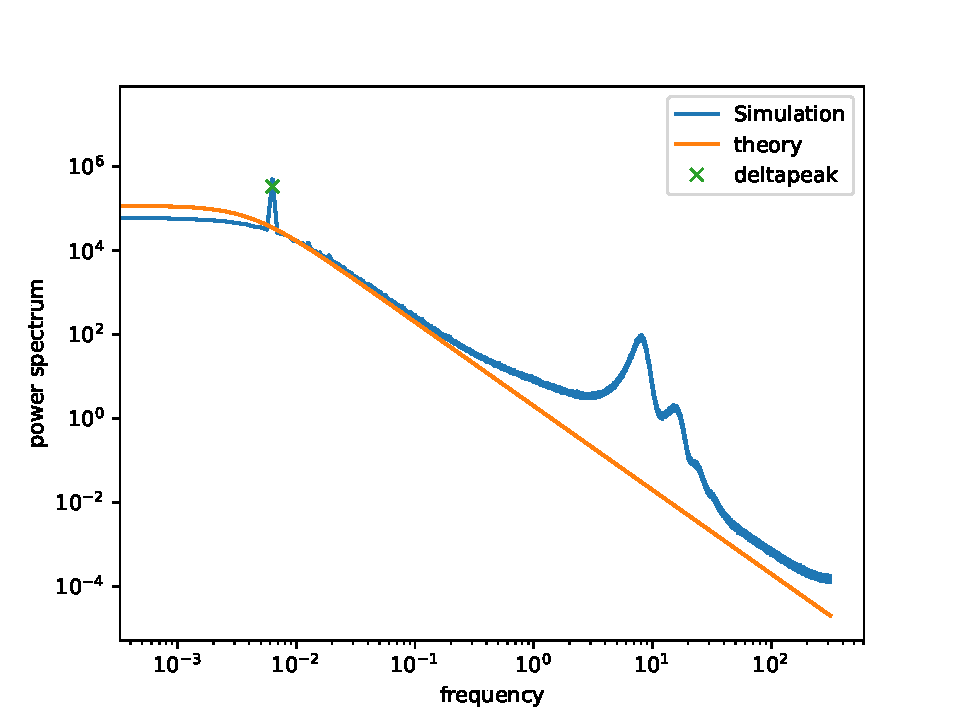
\includegraphics[scale=0.9]{inapik8je1long3011wfom4.pdf}
	\caption{Vergleich Spektrum mit Theorie}
	\label{spectcomp}
\end{figure}

\section{Zwei-Zustands-Theorie} 
F"ur ein System, das von einem schwachen Signal beeinflusst wird, ist das Signal-zu-Rausch-Verh"altnis proportional zu dem Quotienten aus dem Betragsquadrat der Ableitung der (mittleren) Feuerrate $v$ und dem Diffusionskoeffizient:
\begin{align*}
SNR \propto \frac{|dv/dI|^2}{D_{eff}}
\end{align*}
Der Parameter, der hier die Feuerrate steuert, ist der Bias-Strom $I$. Ausnutzend, dass die Feuerrate im ruhenden Zustand verschwindet, kann man die mittlere Feuerrate mittels der "Ubergangsraten zwischen den Zust"anden \glqq burstend \grqq und \glqq ruhend \grqq , $r_+$ und $r_-$, sowie der Feuerrate im burstenden Zustand, $v_+$ berechnen:
\begin{align*}
\left<v\right>=v_+\frac{r_-}{r_++r_-}
\end{align*}
Die Raten $r_+$ und $r_-$ k"onnen aus Gleichung (3) berechnet werden, sodass
\begin{eqnarray}
\frac{dr_\pm}{dI}=-\frac{\Delta U_\pm' }{Q}r_\pm
\end{eqnarray}
Der Diffusionskoeffizient l"asst sich ebenfalls aus diesen Parametern berechnen:
\begin{align*}
D_{\text{eff}}=\frac{v_+^2 r_+r_-}{(r_++r_-)^3}
\end{align*}
L"asst man eine $I$-Abh"angigkeit von $v_+$ zu, ergibt sich dann f"ur die erste Ableitung der Feuerrate:
\begin{align*}
\frac{dr}{dI}&=v_+\left(\frac{r_-'}{r_++r_-}-\frac{r_-(r_+'+r_-')}{(r_++r_-)^2}\right)+v_+'\frac{r_-}{r_++r_-}\\
&=v_+\left(\frac{r_+r_-'-r_-r_+'}{(r_++r_-)^2}\right)+v_+'\frac{r_-}{r_++r_-}\\
&=v_+\left(\frac{r_+r_-(\Delta U_+'-\Delta U_-')}{Q(r_++r_-)^2}\right)+v_+'\frac{r_-}{r_++r_-}\\
&=\frac{r_-}{r_++r_-}\left(v_+\frac{r_+(\Delta U_+'-\Delta U_-')}{Q(r_++r_-)}+v_+'\right)
\end{align*}

Also ist
\begin{eqnarray}
SNR\propto S=\frac{|dv/dI|^2}{D_{eff}}=\frac{r_-(r_++r_-)}{r_+}\left(\frac{r_+(\Delta U_+'-\Delta U_-')}{Q(r_++r_-)}+\frac{v_+'}{v_+}\right)^2
\end{eqnarray}
wobei hier die Abk"urzung $S$ eingef"uhrt wurde, um den sperrigen Ausdruck des Quotienten in Zukunft vermeiden zu k"onnen.
Zun"achst bietet es sich an, zu untersuchen, welches Verhalten dieser Ausdruck f"ur $Q\rightarrow0$ zeigt.\\
Fall 1: $\Delta U_+<\Delta U_-$. Im limes gilt dann $r_+>r_-$, sodass $r_+$ in den gemeinsamen Summen dominiert. Es bleibt also:
\begin{align*}
\lim_{Q\rightarrow0}S&=\frac{r_-(r_+)}{r_+}\left(\frac{r_+(\Delta U_+'-\Delta U_-')}{Q(r_+)}+\frac{v_+'}{v_+}\right)^2\\
&=r_-\left(\frac{(\Delta U_+'-\Delta U_-')}{Q}\right)^2=0
\end{align*}
Obwohl der Term in der Klammer divergiert, dominiert am Ende der exponentielle Term der "Ubergangsrate. F"ur den Fall der Gleichheit werden die Summen statt durch $r_+$ nun mit $2r_+$ ersetzt, was aber zum gleichen Ergebnis f"uhrt. Damit fehlt nun noch der Fall 3:$\Delta U_+>\Delta U_-$:
\begin{align*}
\lim_{Q\rightarrow0}S&=\frac{r_-^2}{r_+}\left(\frac{r_+(\Delta U_+'-\Delta U_-')}{Q(r_-)}+\frac{v_+'}{v_+}\right)^2\\
&=\frac{r_-^2}{r_+}\left(\frac{v_+'}{v_+}\right)^2
\end{align*}
Das Verh"altnis $r_-^2/r_+$ bildet hier also eine Schwelle. Ist dieses konstant, ist auch das SNR endlich. Ist es kleiner als besagte Konstante, geht der Ausdruck gegen 0, sonst divergiert er. Damit tritt Divergenz ein, wenn der burstende Zustand stark bevorzugt wird, also f"ur einen hohen Bias-Strom. Weiterhin ist der Grenzwert monoton, es sind also keine (lokalen) Extrema zu erwarten. Bei Gleichheit gilt folgende Relation:
\begin{eqnarray}
\frac{r_-^2}{r_+}=const\leftrightarrow \frac{r_{0,-}^2}{r_{0,+}}\text{e}^{-\frac{2\Delta U_--\Delta U_+}{Q}}=const
\end{eqnarray} 
Die Potentialbarriere ruhend $\rightarrow$ burstend muss also doppelt so gro"s sein wie die Potentialbarriere burstend $\rightarrow$ ruhend.\\
Weiterhin kann dieser Ausdruck nun auf Extrema untersucht werden.\\
Es ist 

\begin{align*}
S'&=\frac{(r_-'(r_++r_-)+r_-(r_+'+r_-'))r_+-r_+'r_-(r_++r_-)}{r_+^2}\left(\frac{r_+(\Delta U_+'-\Delta U_-')}{Q(r_++r_-)}+\frac{v_+'}{v_+}\right)^2\\
&+\frac{2r_-(r_++r_-)}{r_+}\left(\frac{r_+(\Delta U_+'-\Delta U_-')}{Q(r_++r_-)}+\frac{v_+'}{v_+}\right) \\&\cdot \left[\left(\frac{r_+'}{r_+}+\frac{\Delta U_+''-\Delta U_-''}{\Delta U_+'-\Delta U_-'}-\frac{r_+'+r_-'}{r_++r_-}\right)\frac{r_+(\Delta U_+'-\Delta U_-')}{Q(r_++r_-)}+\frac{v_+''}{v_+}-\frac{v_+'^2}{v_+^2}\right]\\
&=\frac{r_+r_-^2(\Delta U_+'-2\Delta U_-')-r_+^2r_-\Delta U_-'}{Qr_+^2}\left(\frac{r_+(\Delta U_+'-\Delta U_-')}{Q(r_++r_-)}+\frac{v_+'}{v_+}\right)^2\\
&+\frac{2r_-(r_++r_-)}{r_+}\left(\frac{r_+(\Delta U_+'-\Delta U_-')}{Q(r_++r_-)}+\frac{v_+'}{v_+}\right) \\&\cdot \left[\left(-\frac{\Delta U_+}{Q}+\frac{\Delta U_+''-\Delta U_-''}{\Delta U_+'-\Delta U_-'}+\frac{\Delta U_+r_++\Delta U_-r_-}{Q(r_++r_-)}\right)\frac{r_+(\Delta U_+'-\Delta U_-')}{Q(r_++r_-)}+\frac{v_+''}{v_+}-\frac{v_+'^2}{v_+^2}\right]
\end{align*}
Da dieser Ausdruck etwas unhandlich ist, m"ussen einige vereinfachte Annahmen gemacht werden:
\begin{align*}
v_+&=a_vI+b_v\\
\Delta U_\pm&=a_\pm I+b_\pm\rightarrow\Delta U_\pm'=a_\pm,\Delta U_\pm''=0
\end{align*}
Hier muss betont werden, dass $a_v>0$,$a_+>0$ und $a_-<0$ ist, da eine Erh"ohung von $I$ den burstenden Zustand bevorzugt.\\ 
Dann reduziert sich der Ausdruck etwas:
\begin{align*}
S'&=\left[\frac{r_+r_-^2(a_+-2a_-)-r_+^2r_-a_-}{Qr_+^2}\left(\frac{r_+(a_+-a_-)}{Q(r_++r_-)}+\frac{a_v}{v_+}\right)\right.\\
&+\left.\frac{2r_-(r_++r_-)}{r_+}\cdot \left[\left(-\frac{a_+}{Q}+\frac{a_+r_++a_-r_-}{Q(r_++r_-)}\right)\frac{r_+(a_+-a_-)}{Q(r_++r_-)}-\frac{a_v^2}{v_+^2}\right]\right]\\
&\cdot\left(\frac{r_+(a_+-a_-)}{Q(r_++r_-)}+\frac{a_v}{v_+}\right)
\end{align*}
Als erstes wird der Faktor in der letzten Zeile betrachtet:
\begin{eqnarray}
0=\frac{r_+(a_+-a_-)}{Q(r_++r_-)}+\frac{a_v}{v_+}\rightarrow\frac{r_+}{r_++r_-}=-\frac{a_v}{v_+}\frac{Q}{a_+-a_-}
\end{eqnarray}
Da aus den oben beschriebenen Bereichen der Parameter folgt, dass die rechte Seite strikt negativ ist, w"ahrend die linke nur positiv sein kann, l"asst sich daf"ur keine L"osung finden.\\
Da sich die Raten $r_\pm$ aus Exponentialfunktionen zusammensetzen, kann f"ur den zweiten Teil der Gleichung keine analytische L"osung gefunden werden. Stattdessen kann jedoch der Limes $Q\rightarrow0$ betrachtet werden. "Ahnlich wie vorhin gibt es 3 F"alle zu unterscheiden.\\
$\Delta U_+<\Delta U_-$ bzw $r_+>r_-$:
\begin{align*}\nonumber
S'&=-\frac{a_-r_-r_+^2}{Qr_+^2}\left(\frac{r_+(a_+-a_-)}{Q(r_+)}+\frac{a_v}{v_+}\right)+\frac{2r_-(r_+)}{r_+}\left[\left(-\frac{a_+}{Q}+\frac{a_+r_+}{Q(r_+)}\right)\frac{r_+(a_+-a_-)}{Q(r_+)}-\frac{a_v^2}{v_+^2}\right]\\
&=-\frac{a_-r_-}{Q}\left(\frac{a_+-a_-}{Q}+\frac{a_v}{v_+}\right)+2r_-\left[\left(-\frac{a_+}{Q}+\frac{a_+}{Q}\right)\frac{a_+-a_-}{Q}-\frac{a_v^2}{v_+^2}\right]=0
\end{align*}
Da beide Terme mit dem exponentiell abfallenden $r_-$ multipliziert werden geht dr gesamte Ausdruck gegen 0. Auch bei Gleichheit der Raten bleibt eine Rate als Faktor "ubrig, wodurch auch da alles verschwindet. Damit bleibt noch der Fall $\Delta U_+>\Delta U_-$ bzw $r_+<r_-$:
\begin{align*}
S'&=\frac{(a_+-2a_-)r_-^2}{Qr_+}\left(\frac{r_+(a_+-a_-)}{Qr_-}+\frac{a_v}{v_+}\right)+\frac{2r_-^2}{r_+}\left[\left(-\frac{a_+}{Q}+\frac{a_-}{Q}\right)\frac{r_+(a_+-a_-)}{Qr_-}-\frac{a_v^2}{v_+^2}\right]\\
&=\frac{r_-^2a_v}{r_+v_+}\left(\frac{a_+-2a_-}{Q}-\frac{2a_v}{v_+}\right)
\end{align*}
Da im Nenner die Rauschintensit"at auftaucht, kann f"ur diese Gleichung im Limes keine L"osung f"ur $S'=0$ gefunden werden.
\section{Realistisches Modell}
Eine ausf"uhrliche Literaturrecherche hat ergeben, dass die Parameter der Konduktivit"aten um mehrere Gr"o"senordnungen verringert werden m"ussen. Um eine "ahnliche Dynamik beizubehalten, muss dann auch die Zeitkonstante $\tau(V)$ vergr"o"sert werden, da das ganze System nun langsamer geworden ist.
Dies sind die neuen Isoklinen:
\begin{figure}[H]
	\centering
	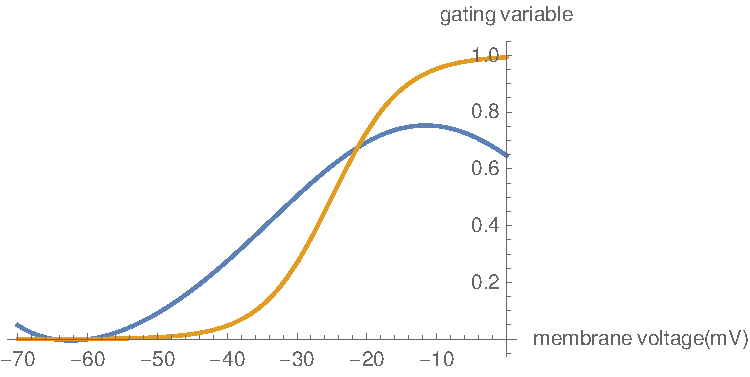
\includegraphics[scale=0.9]{nullclines70Hz.pdf}
	\caption{Isoklinen im realistischen Modell}
	\label{isonew}
\end{figure}
Vorher sahen diese Folgenderma"sen aus:
\begin{figure}[H]
	\centering
	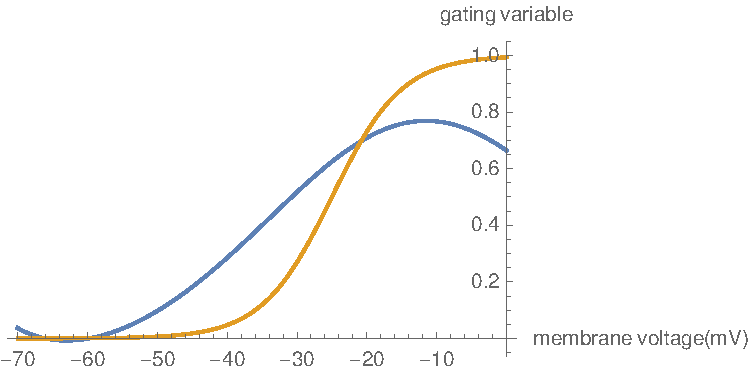
\includegraphics[scale=0.9]{nullclinenew.pdf}
	\caption{Isoklinen im alten Modell}
	\label{isoold}
\end{figure}
Es hat ich also die Amplitude der V-Isoklinen erh"oht, wodurch der instabile Fokus nach rechts verschoben wurde.\\
Die Burstfrequenz hat sich dadurch auf unter 1 Hz reduziert:
\begin{figure}[H]
	\centering
	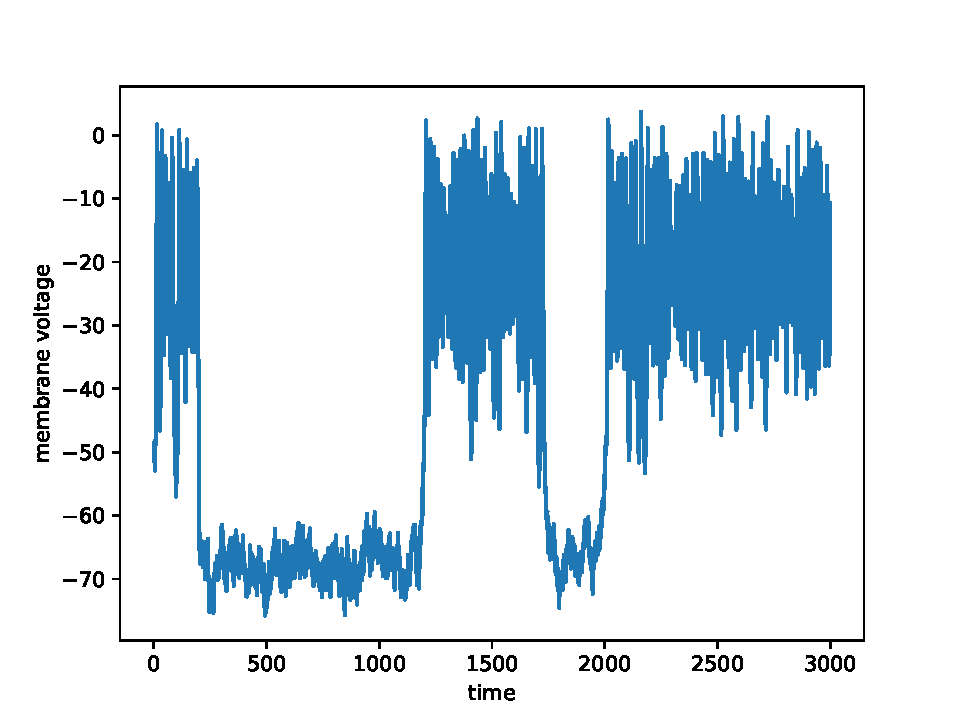
\includegraphics[scale=0.9]{realstate2.pdf}
	\caption{Bistabilit"at der neuen Membranspannung}
	\label{realburst}
\end{figure}
Das Frequenzspektrum zeigt nun deutliche qualitative Ver"anderungen "uber den Bereich des Diffusionskoeffizienten:
\begin{figure}[H]
	\centering
	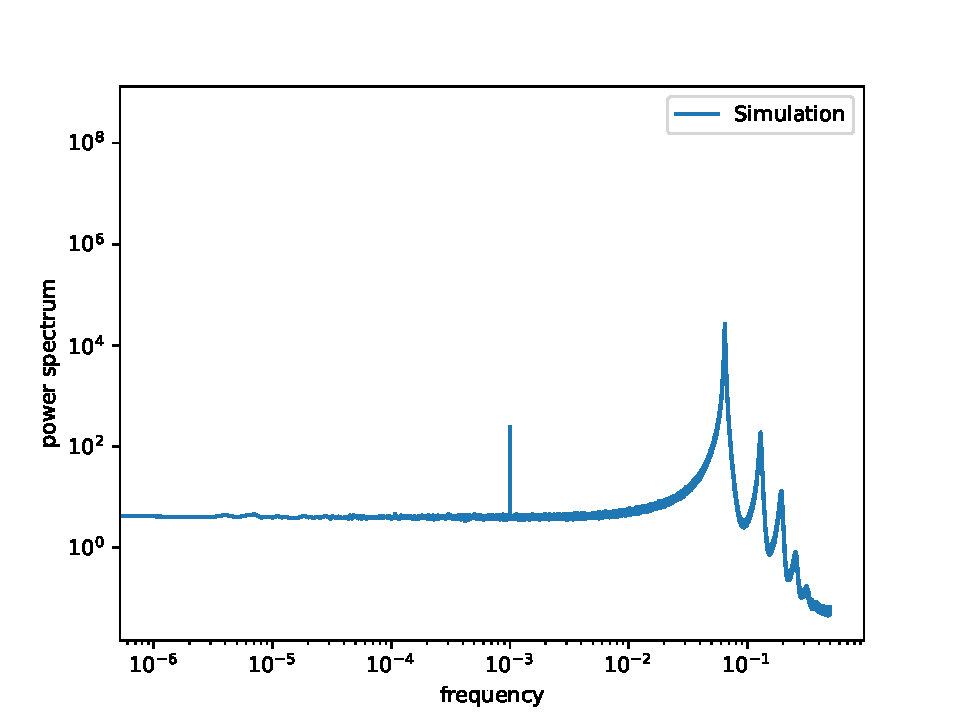
\includegraphics[scale=0.9]{inapikrealfast26jj19.pdf}
	\caption{Frequenzspektrum bei I=0.08, D=0.11}
	\label{deltaspectrum}
\end{figure}
\begin{figure}[H]
	\centering
	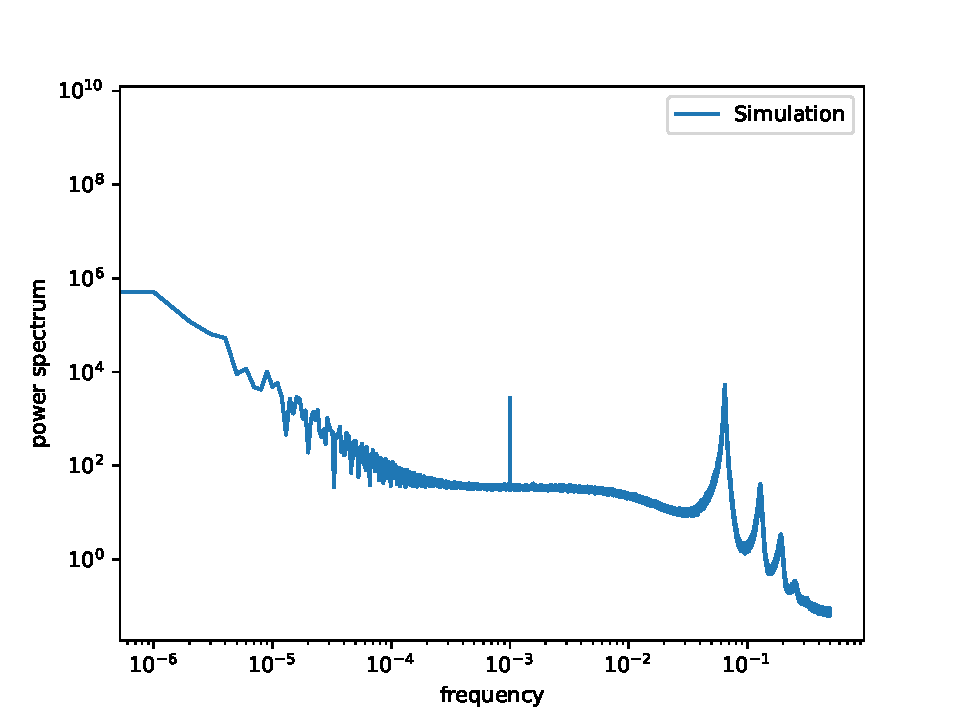
\includegraphics[scale=0.9]{inapikrealfast26jj59.pdf}
	\caption{Frequenzspektrum bei I=0.08, D=0.15}
	\label{deltaspectrum2}
\end{figure}
\begin{figure}[H]
	\centering
	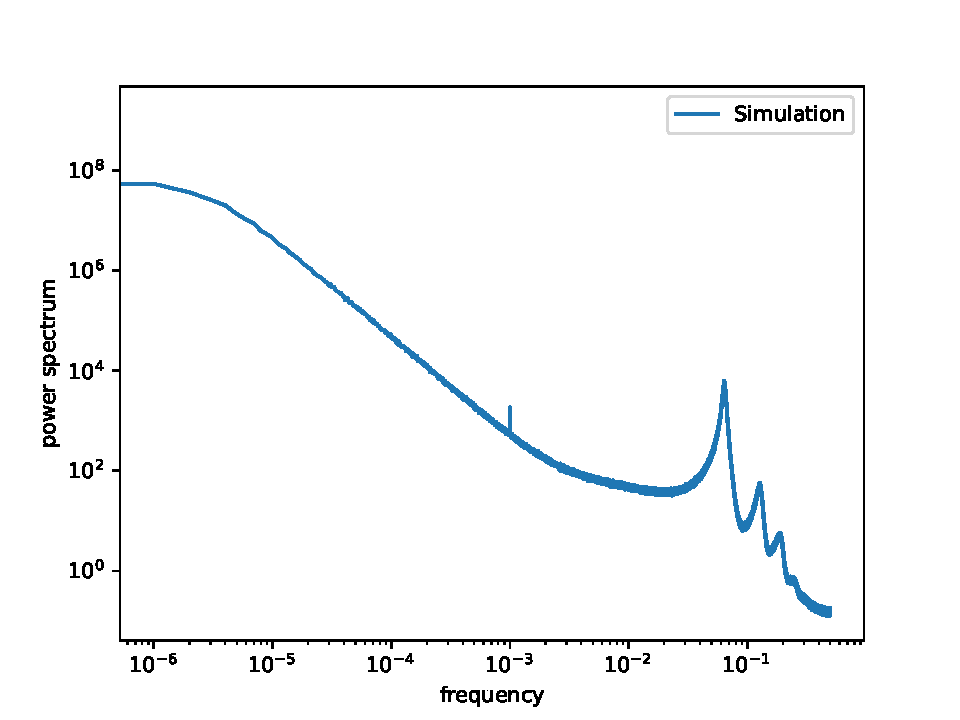
\includegraphics[scale=0.9]{inapikrealfast26jj209.pdf}
	\caption{Frequenzspektrum bei I=0.08, D=0.3}
	\label{deltaspectrum3}
\end{figure}
Es ist bereits mit blo"sem Auge zu erkennen, dass das SNR (bei konstantem Signal) stark abnimmt:
\begin{figure}[H]
	\centering
	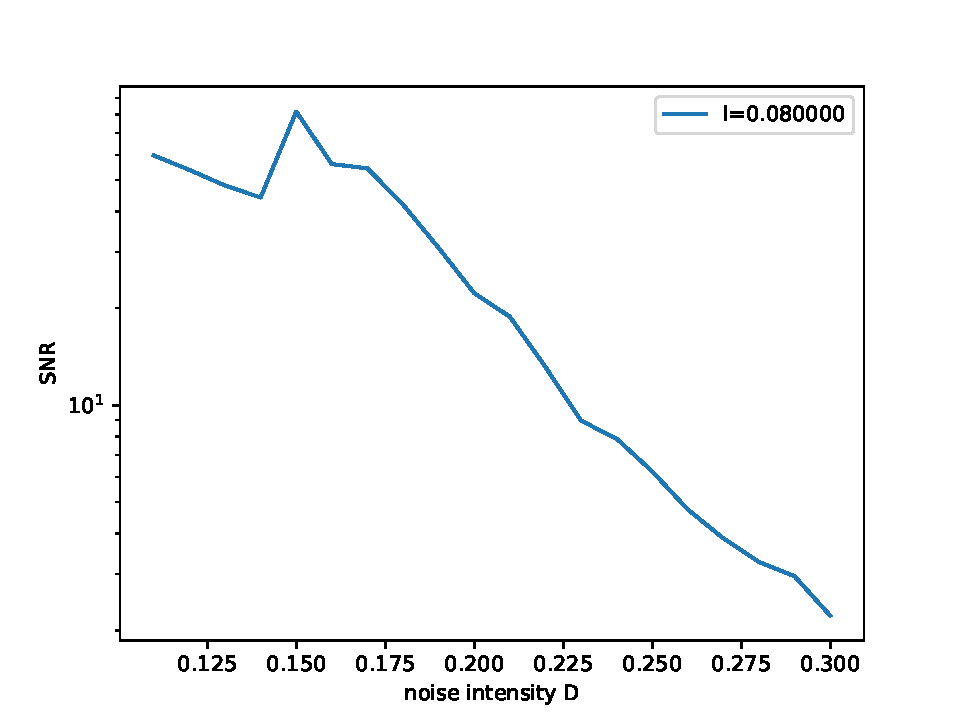
\includegraphics[scale=0.9]{snrdrange26.pdf}
	\caption{Verhalten des SNR bei wechselndem Rauschen}
	\label{snrf1}
\end{figure}
Auch eine Frequenzabh"angigkeit des SNR ist zu erkennen:
\begin{figure}[H]
	\centering
	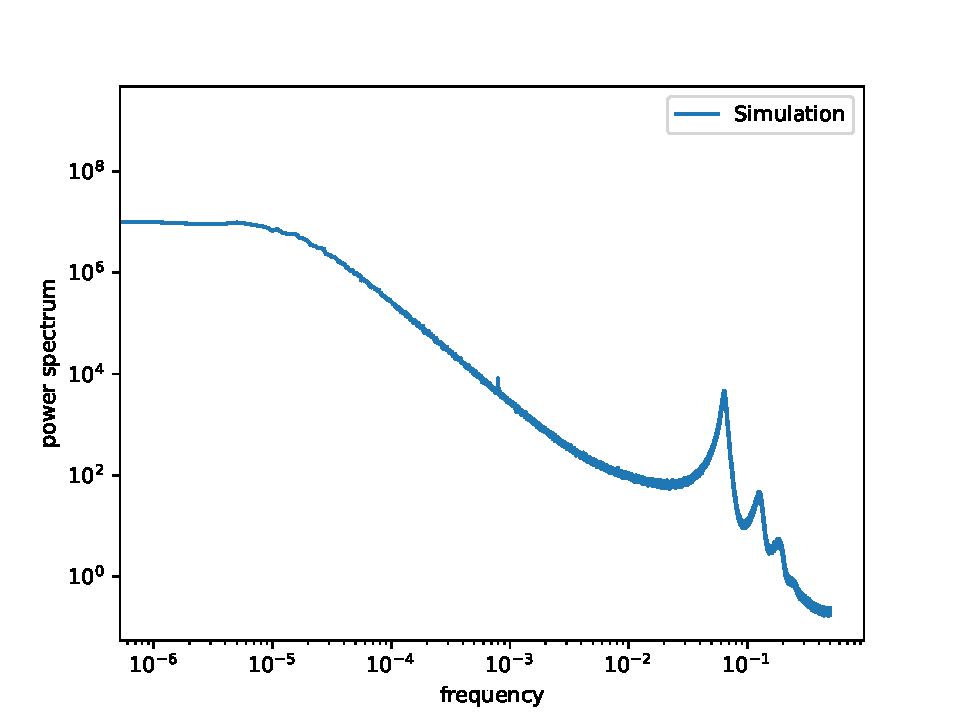
\includegraphics[scale=0.9]{inapikrealfrange26jj304.pdf}
	\caption{Frequenzspektrum bei $I=0.08$,$D=0.4$}
	\label{snrf2}
\end{figure}
\begin{figure}[H]
	\centering
	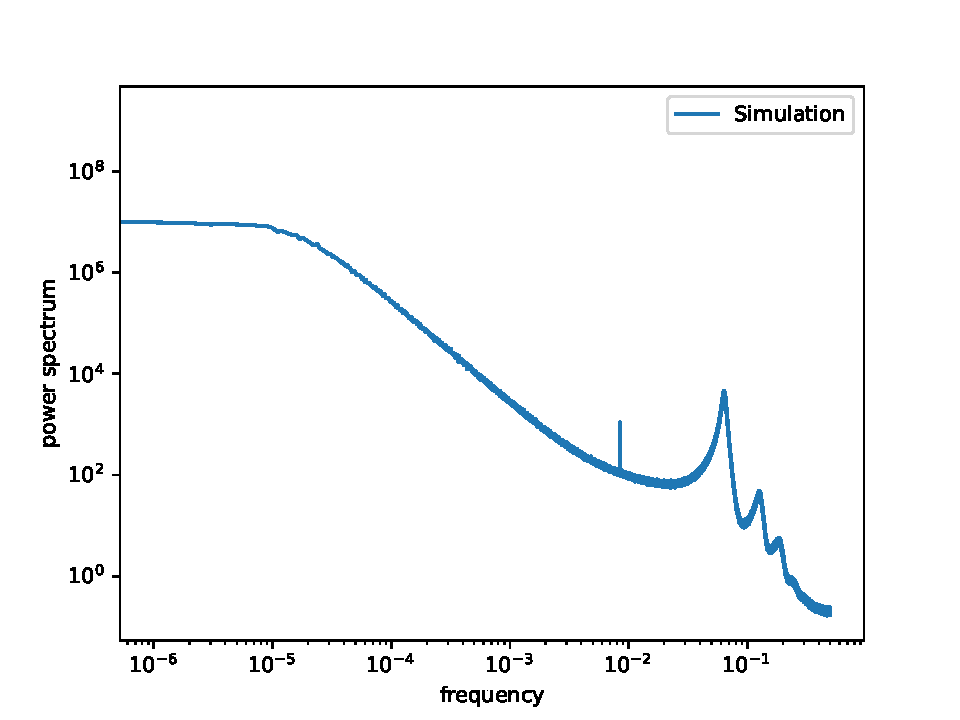
\includegraphics[scale=0.9]{inapikrealfrange26jj3013.pdf}
	\caption{Frequenzspektrum bei $I=0.08$,$D=0.4$}
	\label{snrdrange}
\end{figure}
\begin{figure}[H]
	\centering
	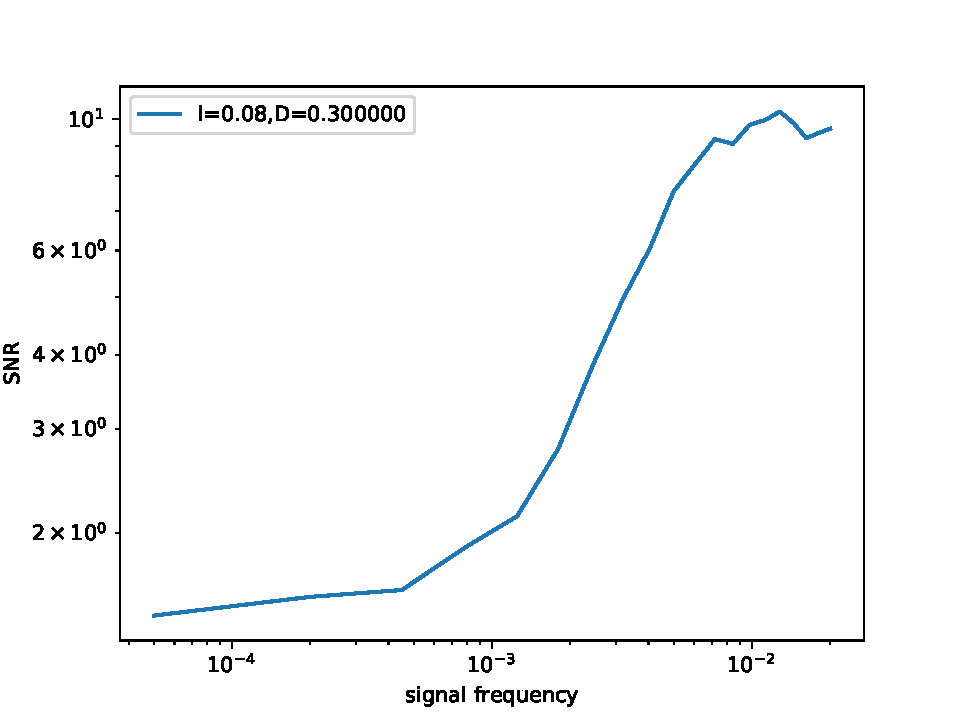
\includegraphics[scale=0.9]{snrfrange2.pdf}
	\caption{Verhalten des SNR bei wechselnder Anregungsfrequenz}
	\label{snfrange}
\end{figure}
Wie erwartet, ist das lokale Maximum bei der Feuerrate im burstenden Zustand bei h"oherem Bias-Strom st"arker ausgepr"agt:
\begin{figure}[H]
	\centering
	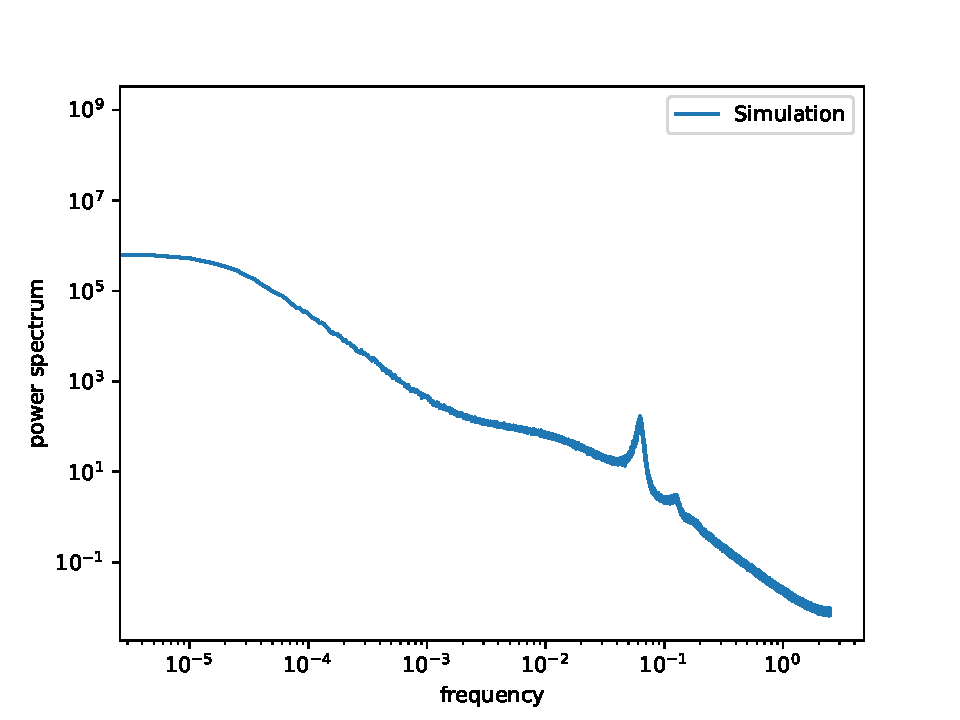
\includegraphics[scale=0.9]{inapikrealfast3jjem3407.pdf}
	\caption{Frequenzspektrum bei I=-0.025, D=0.4}
	\label{sp407}
\end{figure}
\begin{figure}[H]
	\centering
	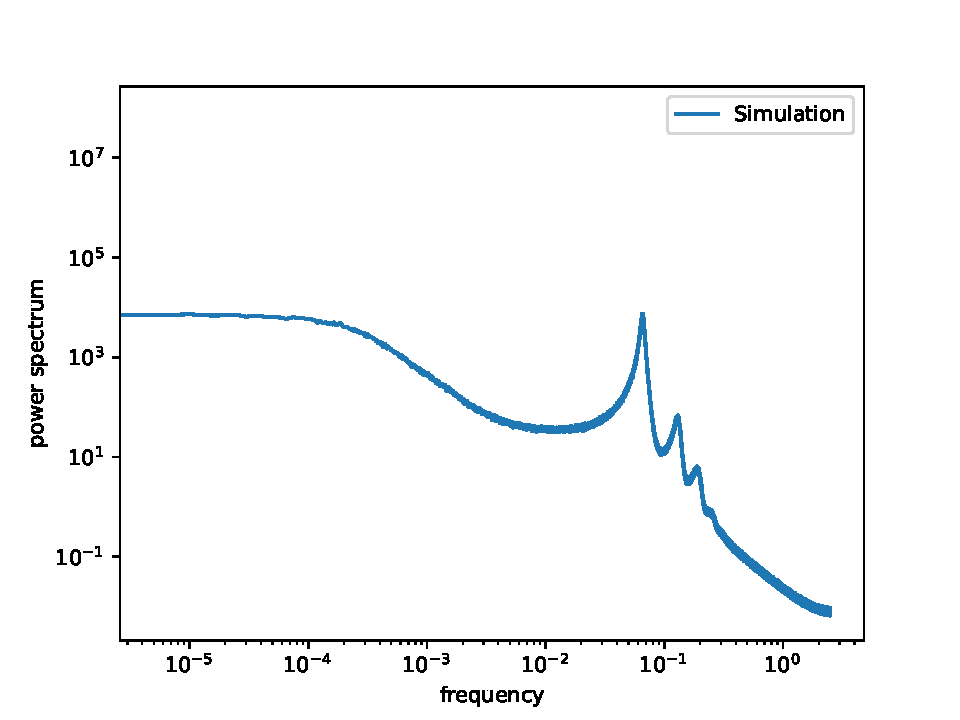
\includegraphics[scale=0.9]{inapikrealfast3jjem34017.pdf}
	\caption{Frequenzspektrum bei I=0.225, D=0.4}
	\label{sp4017}
\end{figure}
Das spiegelt sich auch in den Spektren wider, die aus den Spike-Zeiten erhalten wurden:
\begin{figure}[H]
	\centering
	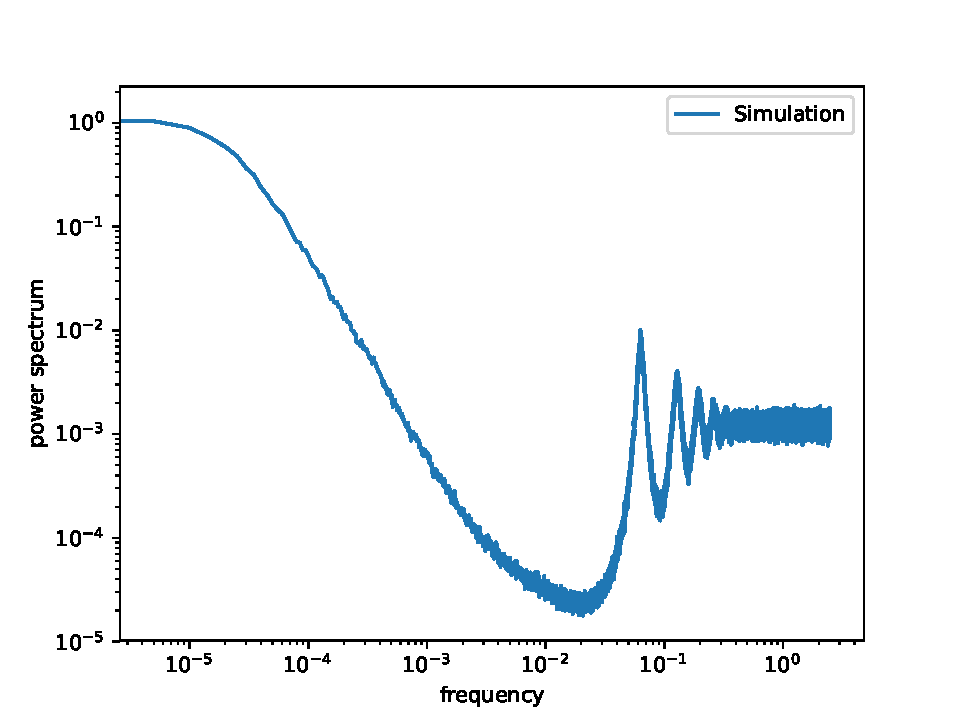
\includegraphics[scale=0.9]{inapikrealfast3jjem3407delta.pdf}
	\caption{Frequenzspektrum aus den Spike-Zeiten bei I=-0.025, D=0.4}
	\label{sp407delta}
\end{figure}
\begin{figure}[H]
	\centering
	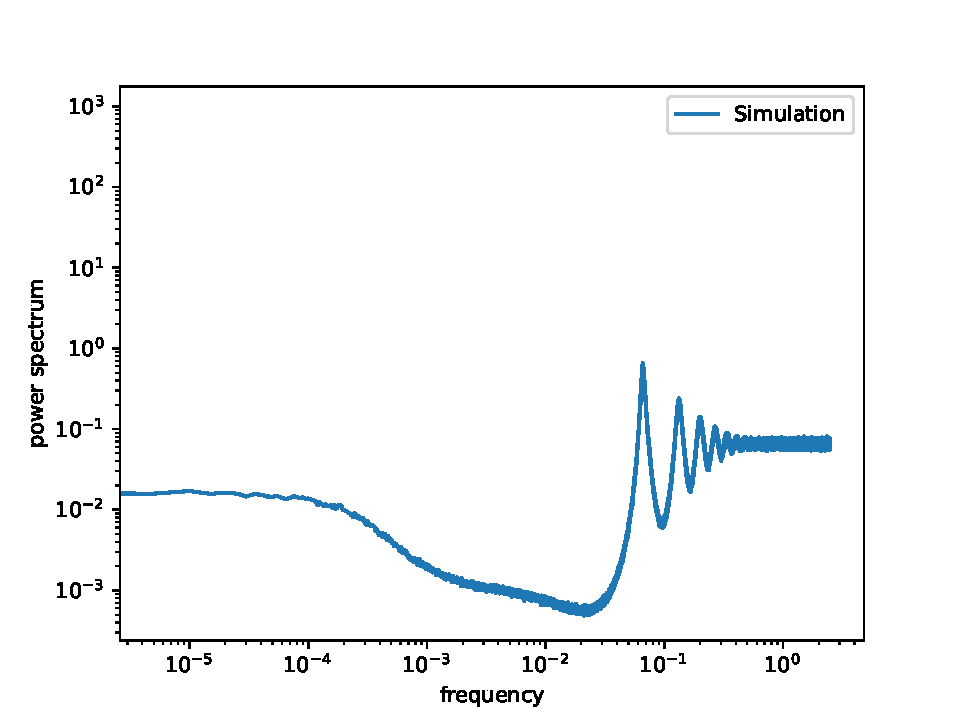
\includegraphics[scale=0.9]{inapikrealfast3jjem34017delta.pdf}
	\caption{Frequenzspektrum aus den Spike-Zeiten bei I=0.225, D=0.4}
	\label{sp4017delta}
\end{figure}
Diffusionskoeffizient, Feuerrate und Fano-Faktor sehen nun folgenderma"sen aus:
\begin{figure}[H]
	\centering
	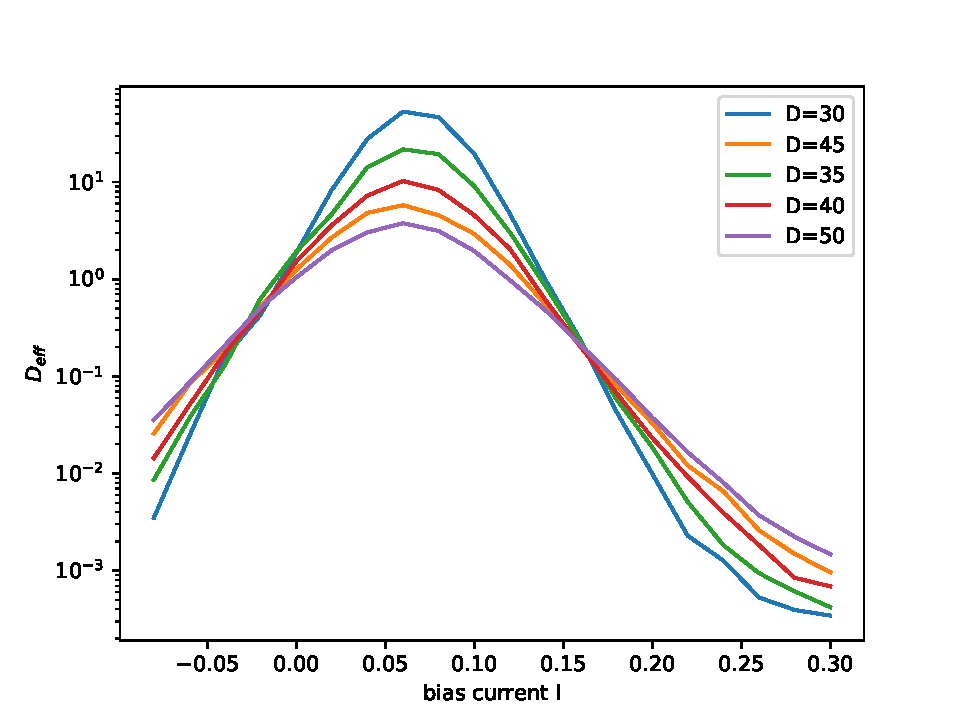
\includegraphics[scale=0.9]{d26.pdf}
	\caption{Neuer Diffusionskoeffizient}
	\label{deff}
\end{figure}
\begin{figure}[H]
	\centering
	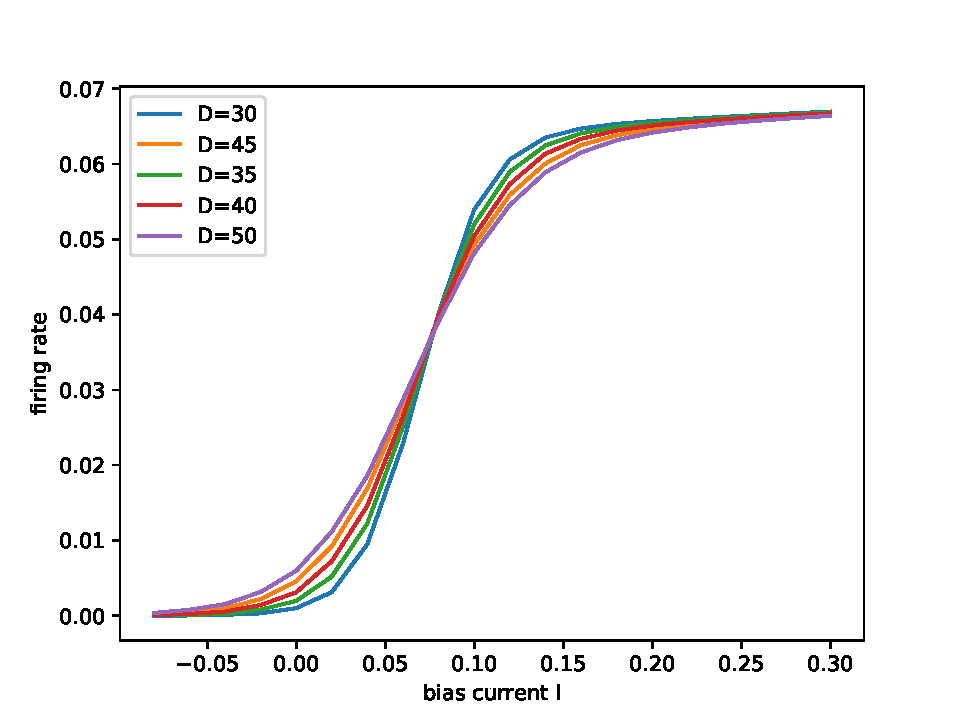
\includegraphics[scale=0.9]{g26.pdf}
	\caption{Neue Feuerrate}
	\label{g}
\end{figure}
\begin{figure}[H]
	\centering
	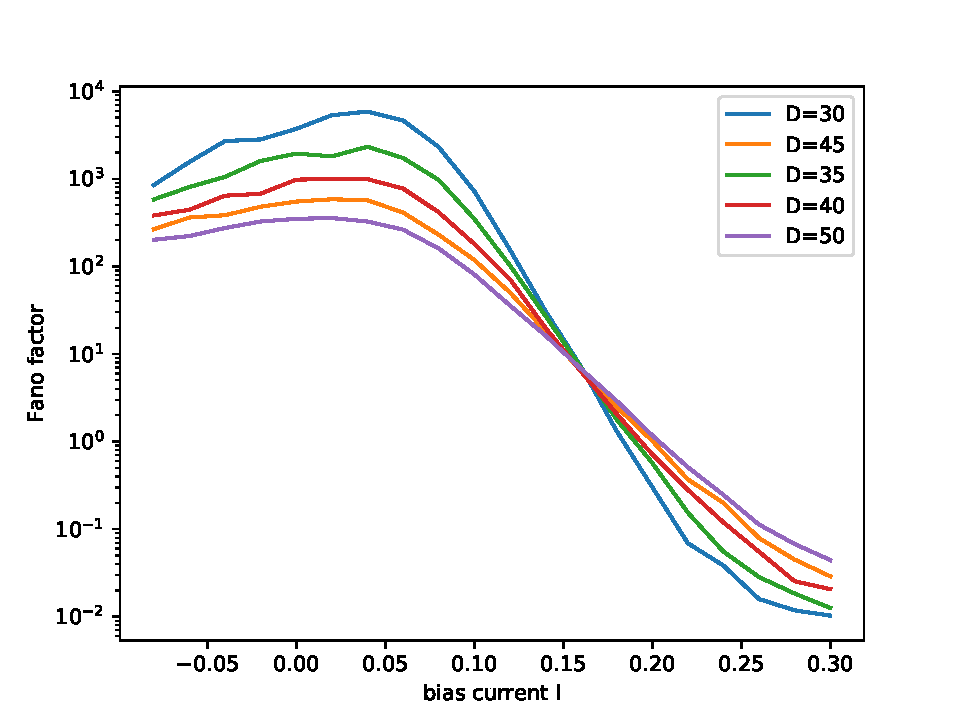
\includegraphics[scale=0.9]{f26.pdf}
	\caption{Neuer Fano-Faktor}
	\label{fano}
\end{figure}
\section{Potentialbarrieren}
F"ur die 3 verschiedenen Rauschintensit"aten, die gerade geplottet wurden, kann man nun wieder Arrhenius-Plots machen und die "Ubergangsraten mit einer Arrhenius-Gleichung fitten:
\begin{figure}[H]
	\centering
	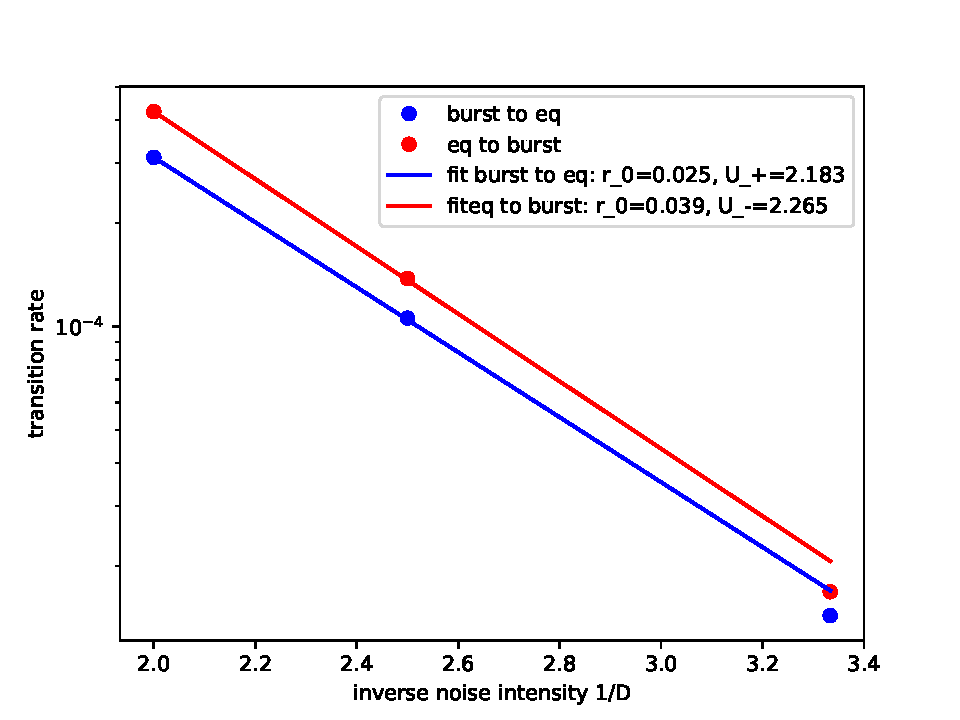
\includegraphics[scale=0.9]{arrheniustotrealfast6jjem2fit1.pdf}
	\caption{Arrhenius-Plot f"ur I=0.075}
	\label{arrh}
\end{figure}
Daraus erh"alt man dann wieder Potentialbarrieren, die sich im betrachteten Bereich ann"ahernd linear verhalten:
\begin{figure}[H]
	\centering
	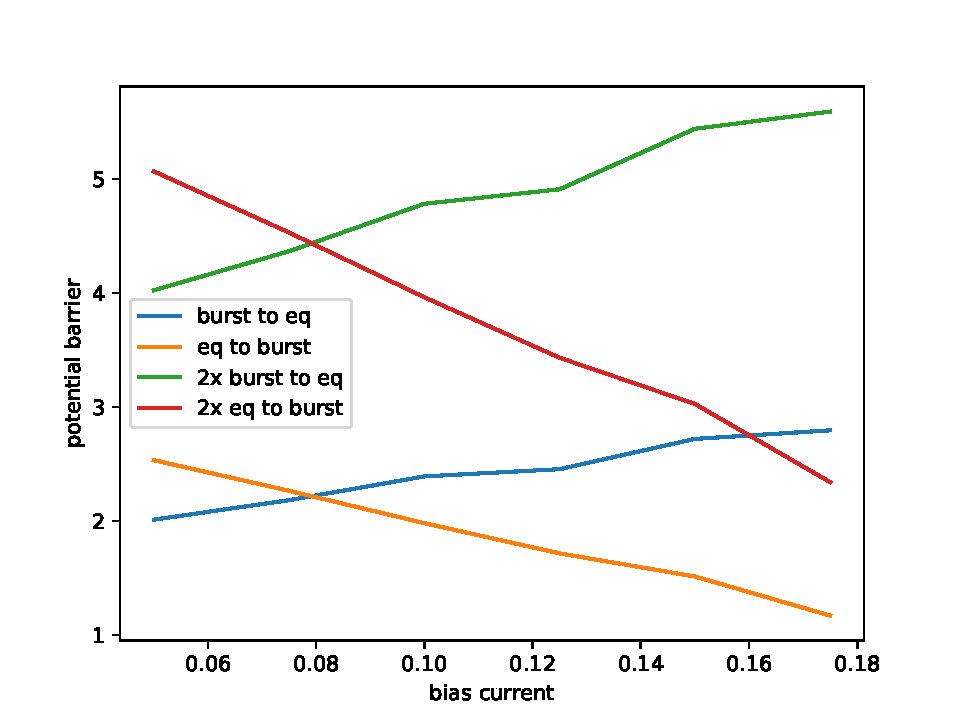
\includegraphics[scale=0.9]{barrier2realfast6jjem2.pdf}
	\caption{Gefittete Potentialbarrieren und ihr doppelter Wert}
	\label{potbar}
\end{figure}
Diese kann man nun in die Zwei-Zustands-Theorie einsetzen und mit den gemessenen Daten vergleichen:
\begin{figure}[H]
	\centering
	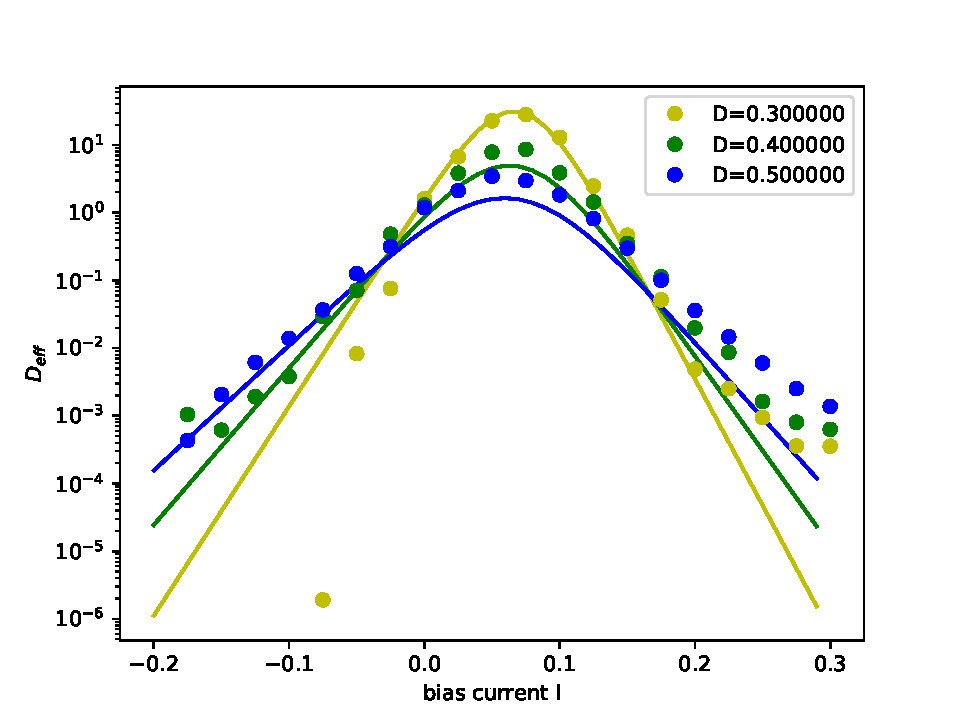
\includegraphics[scale=0.9]{dcompdfrealfast6jjem2.pdf}
	\caption{Gemessener Diffusionskoeffizient und Zwei-Zustands-Theorie}
	\label{deff2st}
\end{figure}
\begin{figure}[H]
	\centering
	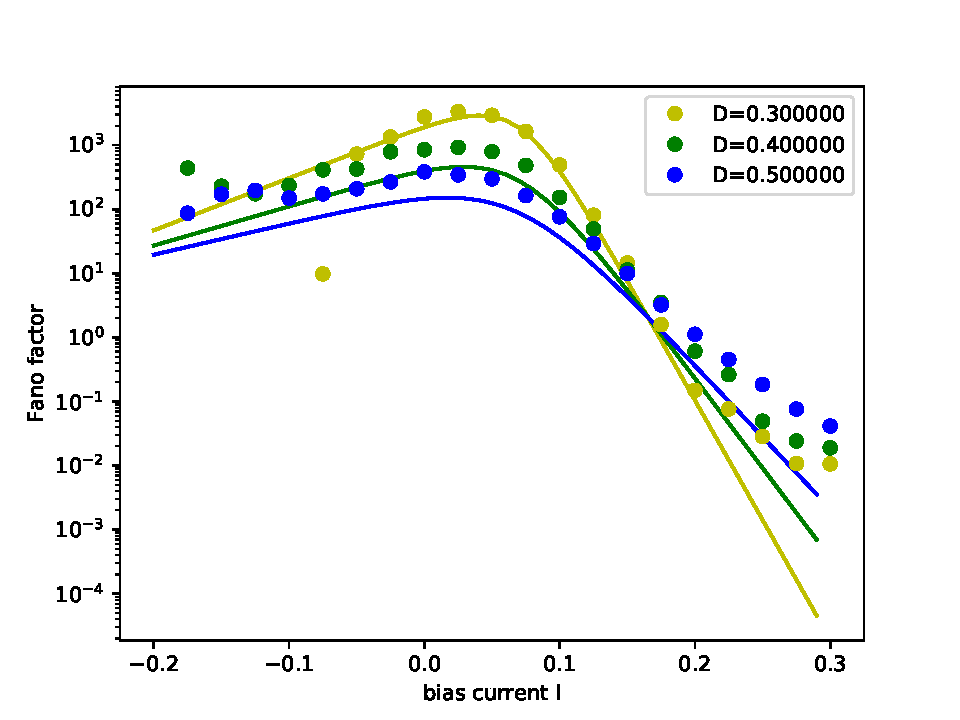
\includegraphics[scale=0.9]{fcompdfrealfast6jjem2.pdf}
	\caption{Gemessener Fano-Faktor und Zwei-Zustands-Theorie}
	\label{fano2st}
\end{figure}
\end{document}